\section{Background}\label{sec:back}
The ideal frequency response of a coupled system, with motor position $\theta_a$ as the output and motor torque $T_{in}$ as the input, can be found in Fig.~\ref{fig:desBode} (left). 
The magnitude plot exhibits a $-40\frac{dB}{dec}$ slope with corresponding phase of $-180^o$.
The frequency response of the system exhibiting TR can be found in Fig.~\ref{fig:desBode} (right). 
It can be noted that at resonance there is a peak. This peak reduces the gain margin of the system. The phase also changes around the resonance which reduces the phase margin.  
We define "\textit{load switching}" as an offset in the $-40\frac{dB}{dec}$ slope that occurs between $\omega_{ar}$ and $\omega_r$, see Fig.~\ref{fig:trBode}.

Contemporary ways of reducing the effects of TR include:
\begin{itemize}
\item Reducing the servo's bandwidth so it does not include the TR frequencies. 
\item Increasing the couplers spring constant $K_c$ via using higher quality and anti backlash mechanical couplers and gearboxes to push the TR frequencies higher. 
\item Using notch filters to reduce the resonant peak. as well as active damping methods\cite{5730488}.   
\end{itemize}

Reducing the bandwidth of the servo means that the designed system will not be able to respond as quickly to an input stimulus. Using higher quality and anti-backlash mechanical couplers and gearboxes will give you greater bandwidth but will also include a higher materials price tag. It is also important to note that the use of notch filters is only useful in systems where the TR does not change. Most systems that have TR present tend to have nonlinear, and time varying, elements, including dynamic loads, that will cause the TR frequency to change thus making the notch filter less effective in the ideal case.  None of the latter methods address the problem of load switching.

Rizzo et. al.\cite{bigley1978resonance} (circa 1978) presented a state feedback technique for, as they describe it, ``\textit{eliminating the destabilizing effect of mechanical resonance in feedback control systems}.''  The goal of their research was to make a wide band high performance closed loop servo system. In their research Bigley and Rizzo found a relationship between the torque, or current, on the DC motor and the velocity of the shaft. They found that when the current is at its maximum the velocity is at a minimum, no matter where the resonance or anti resonance occurs, see Fig.~\ref{fig:re}. Thus feeding back the velocity and torque states would compensate for the effects of TR no matter where it occurs even when the parameters of the system changes.

Sliding mode control (SMC) is a good candidate method to reduce the effects of TR as stated by Korondi et. al.\cite{681228}. This is because SMC is a robust control method that is able to properly control a system even when parameters are not precisely known.   The main idea about SMC is that you are able to make a control that will guarantee the performance of a system in $u$ and $x$, see Fig.~\ref{fig:smcSliding}, within a given error $\psi$ and $\epsilon$ respectively. When using SMC one, or more, parameters are chosen to be unknown. The unknown parameters are given a range that they are able to be between and still have the system perform properly.

\begin{figure}[t]
  \centering
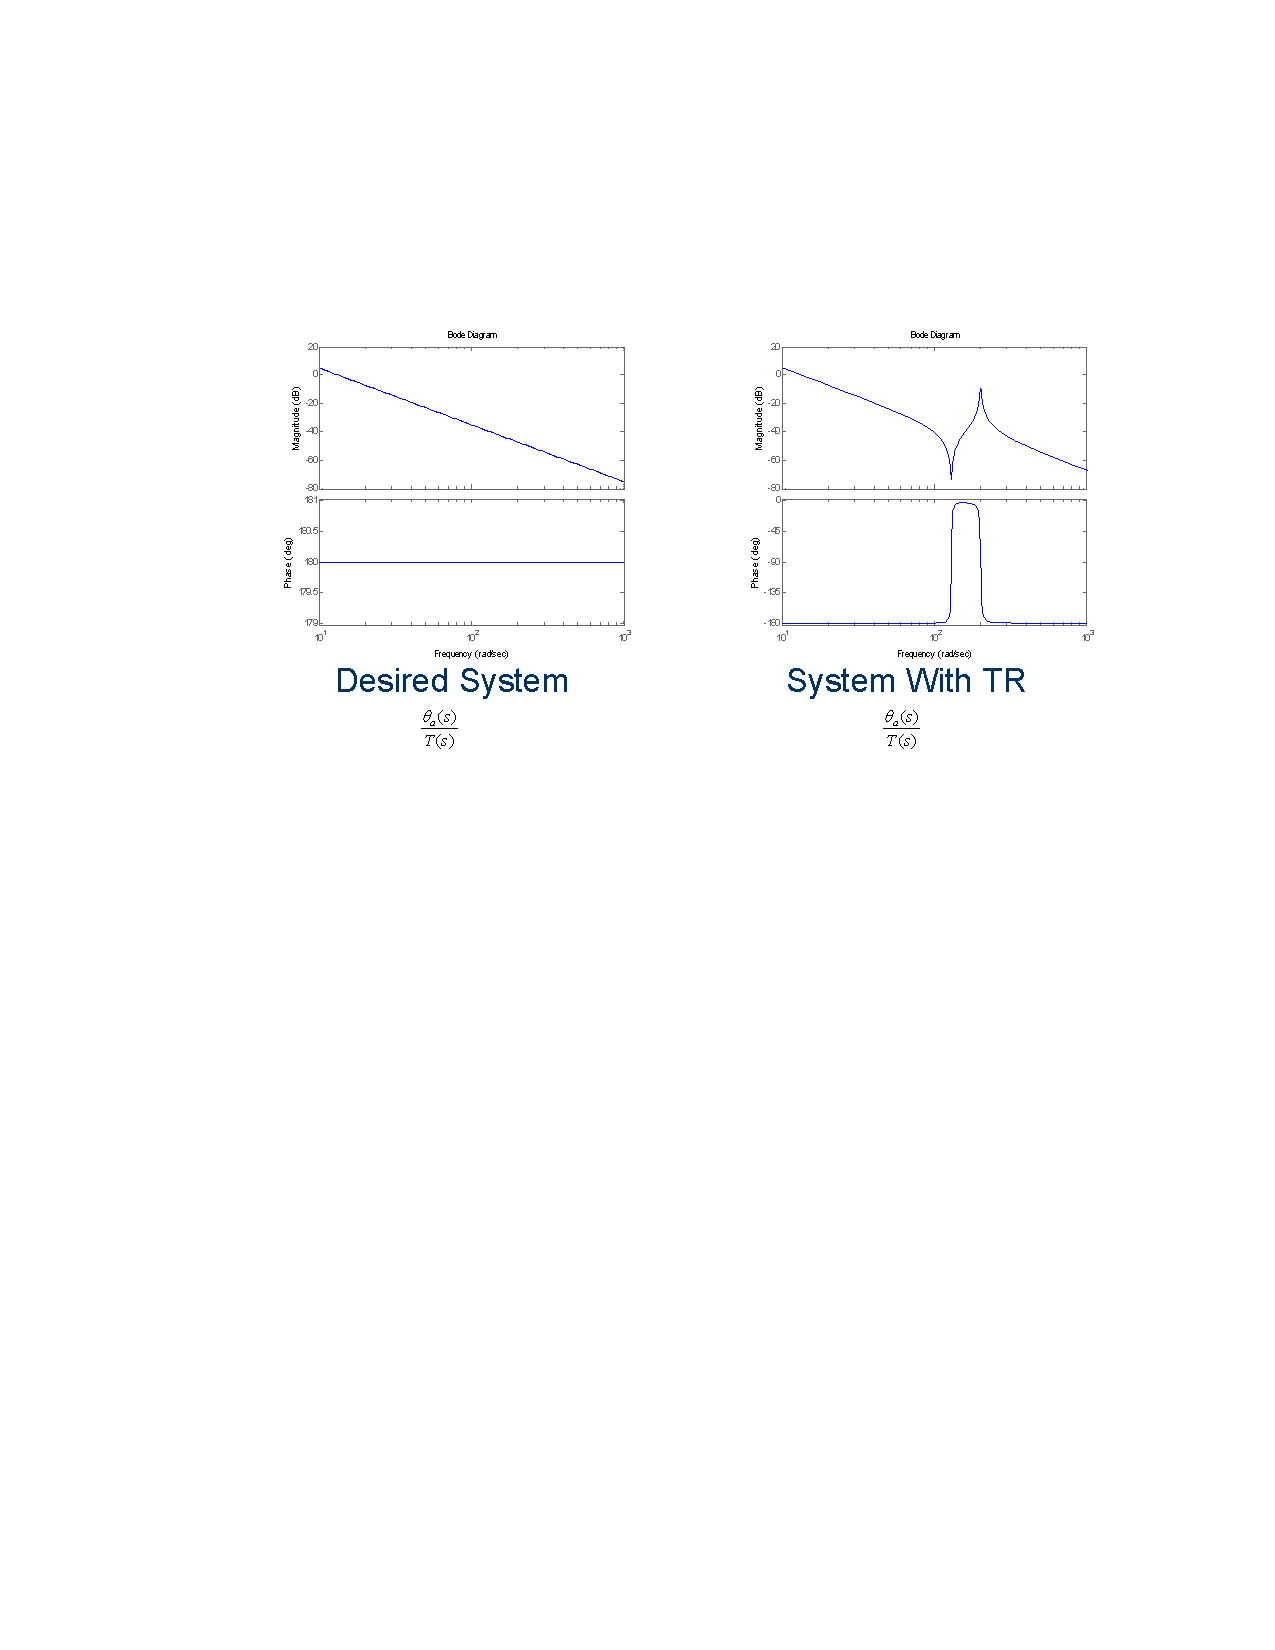
\includegraphics[width=1.0\columnwidth]{./pix/desBode.pdf}
  \caption{Frequency Response of desired coupled system (Left), Frequency response of system
exhibiting TR (Right)}
  \label{fig:desBode}
\end{figure}






